\documentclass[12pt,a4paper,twocolumn]{article}
\usepackage[utf8]{inputenc}
\usepackage[english]{babel}
\usepackage{amsmath}
\usepackage{amsfonts}
\usepackage{amssymb}

\usepackage{graphicx}
\usepackage{float} %precise emplacement float

\usepackage{hyperref}

\usepackage[usenames,dvipsnames]{color}
\usepackage{listings}

\usepackage{natbib}

% Listing settings
\lstset{language=Ruby,
        basicstyle=\scriptsize,
        backgroundcolor=\color{Gray},
        commentstyle=\color{White},
        numberstyle=\scriptsize\color{Black},
        morekeywords={puts, private, public, protected},
        keywordstyle=\color{Blue},
        numbers=left,
        xleftmargin=9pt,
        framexleftmargin=9pt,
        breaklines=true,
        numbersep=1pt,
        tabsize=2}

\title{Comparison of two object-oriented languages: Eiffel and Ruby}
\author{Quentin De Clerck}
\begin{document}
\maketitle
\tableofcontents
\section{Foreword}
This paper is written in an evaluation context of the course Principles of Object-Oriented Programming Languages and has for aim to compare the features of two object-oriented languages. The chosen languages are Eiffel and Ruby. The reasons we decided to choose these two languages is that both have a different type system and philosophies. Eiffel is a statically typed language that aims to produce reusable, extensible and reliable code \cite{meyer2001eiffel}. Ruby is dynamically typed and has for goal to be simple and flexible \cite{rubyAbout}. 
\\
\\
Ruby version: ruby 2.0.0p247 (2013-06-27 revision 41674) [universal.x86\_64-darwin13].
Eiffel version:  EiffelStudio 13 (13.11.9.3542 GPL Edition - macosx-x86-64).
\\
\\
The structure of the paper is divided into two sections. The first section compares for both languages the principal features that are present in most object-oriented programming languages. Since both languages are different in many ways, the second section will focus more on some features that are the most specific to the languages and those that reflects the best the philosophies proper to Eiffel and Ruby. 
\section{General OO concepts}
The aim of this section is to discuss the design choices of the developers of the languages for main concepts of object-oriented languages and to compare the different approaches. 
\subsection{Everything is an object}
Every value in both Eiffel and Ruby are object, even types that are in many languages called primitive types (for example: integers, booleans). Eiffel and Ruby have a similar structure. There is in both languages a class at the top of the hierarchy, this means a class from which every other class in the language inherits its methods. In Ruby this class is called BasicObject\cite{basicObjectDoc} and in Eiffel it is called ANY\cite{meyer2001eiffel}. Besides the ANY class, Eiffel also has the NONE class, which is the class that inherits from every class in the language. Ruby pushes the object-orientation a little bit further with meta-classes. This subject will come back later on in section \ref{sec:metaclass}.
\subsection{Access Control}
In Eiffel there is no possibility to directly perform an assignment on the value of an attribute. The reason for this inability to assign attributes from the outside is because in Eiffel it is impossible to know from the outside of the object if the feature called is a stored or computed value. If there are changes in the implementation, they do not affect the client class by forcing it to change its interface. This concept is called the \emph{uniform-access principle} \cite{meyer2001eiffel, wiki:uniform} and is central in Eiffel. Because it is impossible to know if the expression is an attribute or a function, the only way to change the state of an object is thus to make a procedure than internally modifies the state: a "setter". But there exist a facility to make it look like assignment is directly possible. This mechanism is called assigner command and consists of specifying in the declaration of the attribute which is the related assignment procedure. The assignment of the attribute will be transformed at compile time in the assignment procedure specified in the declaration. They implemented this facility because developers are used to direct access in other programming languages.
\\
\\
An instance variable in Ruby cannot be read/written without calling a method. Thus there is a need for a  "getter" and "setter". The keyword attr\_read, attr\_write and attr\_accessor are syntactic sugar for creating theses methods. Like in Eiffel, the client is unaware if the method is a stored value or a computed one. Thus Ruby also implements the uniform-access principle.
\\
\\
Now there are other mechanisms we have not discussed yet about access controls, namely how to control access to methods to clients outside the scope of the class.
\\
\\
There are three kinds of access controllers in Ruby\cite{wiki:class}: 
\begin{description}
\item[public] accessible without restrictions.
\item[protected] \textit{only} accessible within the class and subclasses.
\item[private] inaccessible \textit{if receiver is explicit} within class and subclasses.
\end{description}
What is meant with "if the receiver is explicit"  is that if the method is called for a specific object, like self or a parameter, then the call will result in an error.By default, every method is public in Ruby and it is possible to change the visibility of the methods at run-time due to the dynamic nature of the language. This dynamic nature will be discussed in a later section.
\\
\\
Eiffel has another approach called \emph{Selective Export}\cite{meyer2001eiffel,accessControlEiffel} . It specifies a list of clients to export, enabling them to get access with the features they were listed for. This approach enables to be very precise about the scope of the features. The different possibilities are:
\begin{itemize}
\item Making a set of features private to the class by specifying that the feature set should not be exported: \{NONE\}.
\item Making a set of features public to every possible client by specifying nothing or by specifying: \{ANY\}.
\item Making a set of features public to a set of clients by specifying the clients, for example \{Class\_A, Class\_B, Class\_C\}. It is possible to specify the current class as client, then every subclass will inherit the feature.
\end{itemize}
This export technology allows to be very specific in the choice of accessible features. Export violations are statically checked by the compiler and thus are detected at compile-time and not at run-time.
\subsection{Inheritance}
Both languages support single class inheritance but only Eiffel supports \emph{multiple inheritance}. However Ruby supports \emph{mixins} which offers the similar possibilities as multiple inheritance.
\begin{figure}[H]
\centering
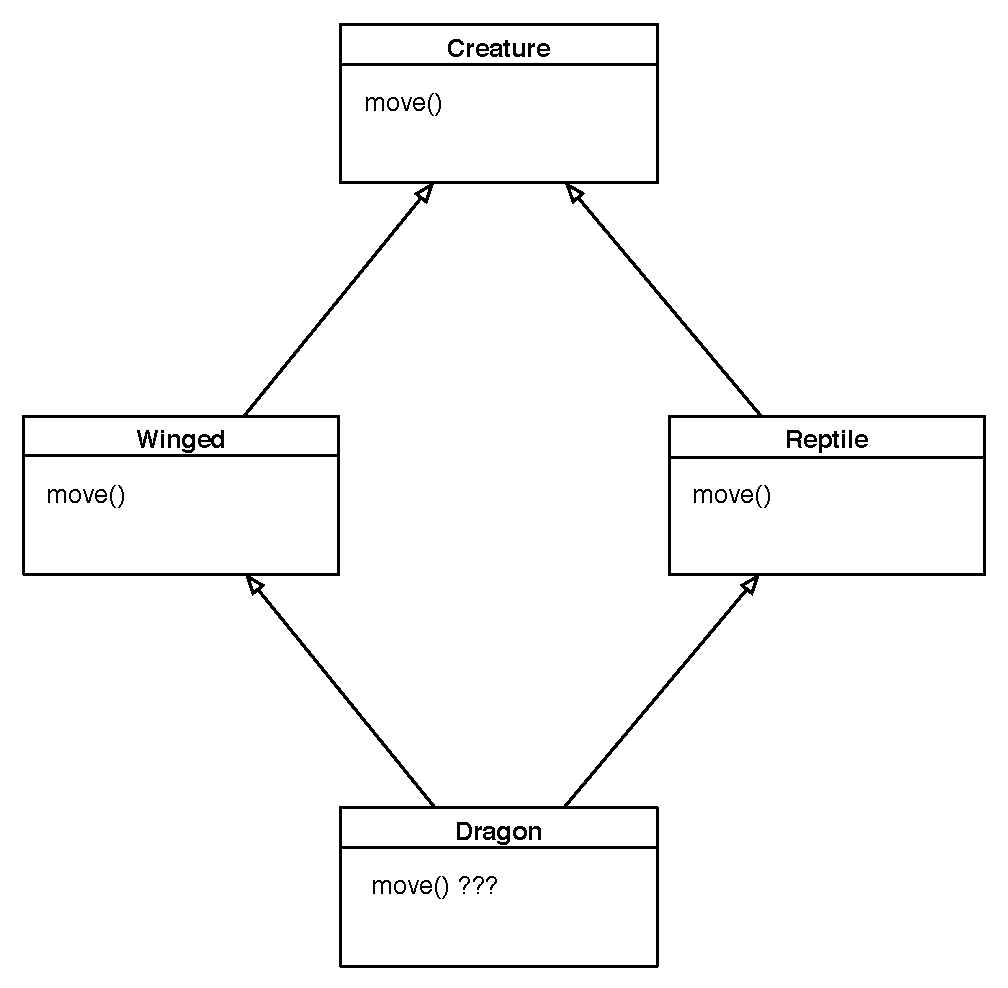
\includegraphics[scale=0.4]{diamond.pdf}
\caption{Example of the diamond problem}
\label{fig:diamond}
\end{figure}
Multiple inheritance is a object-oriented feature where a class inherits from more than one parent class. This can lead to problems like the \emph{diamond problem} depicted in figure \ref{fig:diamond}. The diamond problem arises when two or more parent classes inherit from the same superclass. This will provoke nameclashes in the subclass inheriting from the multiple parents. Eiffel provides a flexible approach to multiple inheritance. It introduces different keywords that enable to adapt the features inherited from the parent classes. The keywords that are provided for feature adaptation are:
\begin{description}
\item[rename] Renames a inherited feature.
\item[export] Changes the export list of the inherited features.
\item[undefine] Removes one of the inherited feature definitions.
\item[redefine] Redefines one of the inherited feature definitions.
\item[select] Selects the feature to use when there are homonyms.
\end{description}
Thus the diamond problem can be easily solved in Eiffel thanks to the provided tools. A simple example for solving the depicted problem in figure \ref{fig:diamond} is to rename the move feature from the Winged class into fly and select the fly feature. Another approach could be to undefine one of the features and selecting the other.
\\
\\
Ruby does not support multiple inheritance,  but a \emph{mixin} \cite{wiki:class, thomas2001programming} can be an equivalent feature. Before explaining what a mixin is it is important to explain \emph{modules} in Ruby. A module is a sort of namespace grouping variables and functions together for obtaining a whole that provides functionalities. Modules cannot be instantiated, their purpose is to add functionality to a class. A mixin allows to include a module as a sort of superclass to the desired class, to mix the module in the class. It is possible to mix more than one module in a class, thus it looks very similar to multiple inheritance. In the example from figure \ref{fig:diamond}, the superclasses could be two modules that implement the different move behaviours. But even if Ruby uses mixins instead of multiple inheritance, the nameclash problem persists. Ruby resolves it automatically by overriding the previous definition, thus it is important for the programmer to be aware of this and give another name to one of the definition if the two method definitions are needed.
\subsection{Polymorphism} 
Polymorphism is a key feature in object-oriented programming languages. Both Ruby and Eiffel support this feature but in a very different conceptual way. Eiffel supports \emph{subtype polymorphism}, it means that Eiffel allows polymorphism only for the types that have a superclass in common. Thus inheritance is primordial for subtype polymorphism. 
\\
\\ 
In Ruby it is also possible to achieve it using inheritance, but this is more a consequence of the mechanism that permits Ruby to support polymorphism. Ruby is dynamically typed and supports a special style of typing namely, \emph{duck typing}\cite{wiki:duck}. Duck typing focusses on the methods of an object instead of its type. If the method is supported by the object it will be called whatever the type or output is. If the method call is not supported, then a run-time error is returned. Duck typing is the concept used for polymorphism in Ruby allows thus polymorphism without inheriting from a superclass. It is trivial why polymorphism also works with inheritance in Ruby, classes that inherit from a superclass inherit its methods and duck typing focusses on the presence of methods.
\\
\\
So even if both languages support polymorphism, their approach is completely different. Polymorphic calls are dependent of the type of objects in Eiffel and in Ruby they are dependent of the presence of the method. From a software engineering point of view it is logical that Eiffel focusses on the subtype polymorphism. First it is statically typed, thus there should be a specific type declared for the variable or parameter. However, this could be resolved with a keyword that instructs the compiler that a variable should be dynamically typed (like the "dynamic" keyword of C\#). Second and most importantly, this sort of solution is not in the philosophy of the Eiffel language. One of the goals of Eiffel is to produce software that is reliable and maintainable. If duck typing should be adapted in Eiffel then it would be only reliable if the programmers know exactly which type of objects will passed to the methods. The maintainability of the software would also be tricky, imagine that a method call changes of name in one of the classes, with duck typing it would not be clear that this method was used in a polymorphic call and by changing its name the programmer introduces errors that can be tedious to resolve. Thus it is important to be aware of the methods that are used in a polymorphic context when a language supports duck typing. Subtype polymorphism in a statically typed language is a much more reliable mechanism because the polymorphic calls are only possible for a restricted set of types and eliminate a lot of possible failures. It is also more easily maintained, because it is checked at compile time that every class implements the method. In Ruby's case, it is also logical that duck typing is used and not subtype polymorphism. First, subtype polymorphism is implicit with duck typing. Second, Ruby is dynamically typed, which means the types are known at run-time. This implies that there would be no secure way to ensure that the method call is applied on a particular class hierarchy. Perhaps it could be achieved with a kind of type cast for the desired superclass. But then it would still return a run-time error when the types are not correct, like it does when the method is not defined for an object. This is much more restrictive and goes also against the philosophy of Ruby which is simplicity and flexibility.
\section{Language-specific Features}
While the first section enumerates differences in general object-oriented concepts, this section focusses more on features that characterize the languages. The aim is not make an exhaustive list of features but more to pick some that really show the purpose and philosophy of the languages.
\subsection{Eiffel}
The goal of Eiffel is to provide rather a method that guides the programmer in software development than only a language for programming. It focusses on some the whole software development process and on the quality of the software. 
\subsubsection{Design by Contract}
If there is one language specific feature that is essential in Eiffel, then this concept is \emph{Design by Contract}\cite{meyer2001eiffel, eiffelEssentials}. The idea is that every system has interacting components and that their cooperation should follow some strict specifications (the contract) that settle the obligations and benefits for both client and supplier. The obligations have to be satisfied before feature calls. They are called \emph{preconditions} and are introduced by the \emph{require} keyword. The benefits describe what the result should be if the precondition was met. Benefits are thus \emph{postconditions} and can be specified using the \emph{ensure} keyword. Every contract also include \emph{class invariants}, which are conditions that have to be ensured during the lifetime of an object, including at its creation. Class invariants are specified after the \emph{invariant} keyword. These are the three main categories of contracts and are implemented using assertions. Each assertion may be tagged, it is not mandatory and does not influence the contract but it is helpful for debugging and provides extra documentation. Since assertions are boolean expressions, it is possible to formulate them in function calls. This enables to express more complex conditions.
\\
\\
There are still three other types of assertions: 
\begin{itemize}
\item Instruction check: checks if a certain condition is respected at a specific moment during the execution.
\item Loop invariants: states that some conditions have to be ensured when exiting the loop.
\item Loop variant: make sure the loop is finite by decreasing an integer expression at each loop iteration and check that the integer stays positive.
\end{itemize}
Even if Design by Contract is not mandatory to use when developing in Eiffel, it is strongly encouraged because it has many benefits. It is a method that helps the developers for designing and implementing correct software in first instance. They push the developers to think about specifications for the code to write. It has already been pointed out that using tags for assertions are useful for code documentation and debugging. Contracts serve also to generate automatically documentation in Eiffel, this means that the documentation is always up-to-date. Design by Contract is thus a methodology that encourage the programmer to think about the code, to write specifications down about the code and to design the code such that the specifications are fulfilled. This is thus a great feature for reliability and maintainability of the software.
\\
\\
There exist libraries in many programming languages that offers Design by Contract, even for \href{https://github.com/egonSchiele/contracts.ruby}{Ruby}. A basic implementation of Design by Contract in Ruby \ref{rb:contract} has been implemented for this paper. It uses reflection in order to get information about the variables and metaprogramming for evaluating the expressions passed to the require, ensure and invariant clauses.
\subsection{Void-safety}
\emph{Void-safety}\cite{voidSafety} is a language feature that protects the software from run-time errors caused by method calls to void references. References are used for accessing objects in object-oriented programming languages. This can lead to problems when the reference is Void (or null in other languages).
\\
\\
Eiffel is statically typed and thus can ensure that a feature will be applied at run-time to the correct object. But nothing ensures that the object will exist when the feature will be executed. With Void-safety the compiler can give the assurance that an object will be attached to the reference whenever the feature is executed. In other words, the compiler analyses the code statically and ensures that feature calls are valid only if the feature executes a call on an attached object and not to Void.
\\
\\
There are patterns that check if a variable is void-safe. The \emph{Certified Attachment Pattern} (CAP) checks if a local variables or formal parameters is void. The \emph{attached syntax} takes a step further. It is another sort of CAP that checks if the object is attached and provides a safe access to the objects that are attached as class attributes. Eiffel introduced two kind of types in order to assure the void-safeness of the software:
\begin{description}
\item[Attached Type: ] The compiler will prevent a variable of an attached type to be set to Void.
\item[Detachable Type: ] Theses variables may be set to Void. Thus direct access to detachable typed variables is never void-safe.% which means that CAPs and attached syntax are only needed on them. 
\end{description}
It is also important to note that it is impossible to assign a detachable variable to an attached one, but the opposite is possible. The creation procedure is responsible for ensuring that all the attributes of an attached type are set after the creation. 

This is a feature that improves the reliability of the produced software and shows again that Eiffel's primary concern is to enhance the software quality. In Ruby there is nothing like void-safety. Void safety is achieved at compile time and Ruby is an interpreted language, thus there is no way to make it void safe except by checking if the object is the nil object.
\subsection{Ruby}
Ruby is a programming language known for being very object-oriented and for its simplicity. It is also very flexible like duck-typing already attested in previous section.
\subsubsection{Open Classes}
In Ruby it is always possible to add new methods to an existing class, the class definitions can at any moment be opened for modifications. Even built-in classes are can be adapted. Adding or modifying content at run-time to an already existing class definition without altering the source code is known as \emph{monkey patching} \cite{wiki:monkey}. 
\\
\\
Monkey patching can be useful for different applications like extending or modifying the behaviour of an object at run-time from a third-party software without changing the source code. This enables for example to reuse existing code and adapt it in different files with different behaviours.
\\
\\
In first instance this feature seems really helpful because it gives the possibility to the developer to adapt code when needed. For example, as workaround to a bug by implementing a specific solution in this part of the code. But with great power comes great responsibility. Monkey patching can lead to bugs that break the code. If the source code changes, it is possible that the patch behaves differently because it makes assumptions on the code that do not hold anymore. Different patches for the same method create conflicts and one patch will override the other. Thus it is important to be aware of the patches and save the implementation of a method if necessary by renaming it with an alias. It is also important to document the patches and method that are patched, this can prevent confusion if one forgets or does not know about the existing patches and does not understand why the code does not act like expected.
\\
\\
To summarize, open classes is thus a language feature that offers a lot of modularity and flexibility. It enable to extend and reuse third-party code in a simple way. This is certainly why this feature has been added in Ruby. But it is very important to note that open classes are in conflict with the principle of encapsulation. Every method can be accessed with open classes, even private methods and they can  be changed into public ones. It is thus really important of not abusing of this feature. 
\subsubsection{Metaclass model}
\label{sec:metaclass}
% http://en.wikipedia.org/wiki/Metaclass
A metaclass is a special class that has classes as instances. It defines thus methods that every class and its instances should have. When asking to a class in Ruby from which class it is an instance, it will always return the class Class. This is logical since every class should inherit the methods defined in it. Thus the only metaclass in Ruby is thus the class Class.
\\
\\
But lets look the meta-system a little bit more in details. In Ruby there exist meta-objects called \emph{eigenclasses}. Every object has its own eigenclass. Because classes are also objects in Ruby, they also have eigenclasses. And what is interesting is that eigenclasses also have eigenclasses. This is recursive and goes on forever. Thus there are three sorts of eigenclasses: eigenclasses for objects and for classes. 
\\
\\
But what is the usefulness of theses eigenclasses? When an instance method is defined, it is stored in the class. When a class method is defined, it is stored in the class' eigenclass. Thus the eigenclass serves to store class variables and class methods. Eigenclasses of objects are useful if the developer wants that this particular object has a different behaviour than the other objects of the same class. Specialized method for this object will be stored in the eigenclass of the object. And finally, Eigenclasses of eigenclasses do not store any method or data, thus the reason of there existence is for conceptually correctness. 
\begin{figure}[H]
\centering
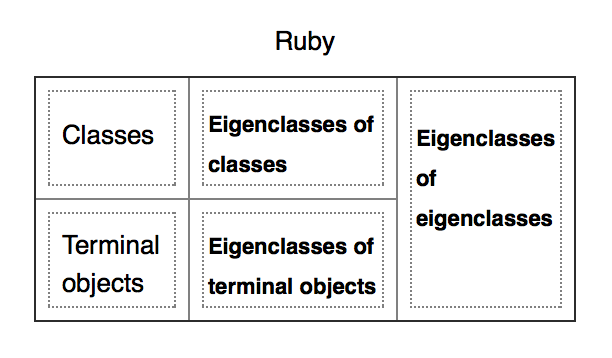
\includegraphics[scale=0.5]{Ruby.png}
\caption{The Ruby metaclass model. Image from Wikipedia}
\label{fig:metaclass}
\end{figure}
The method lookup mechanism works thus as follows: 
\begin{enumerate}
	\item A method is called on the object
	\item The method is looked up in the methods of the object's eigenclass
	\item If the method is not found, the lookup continues in the class of the object
	\item If the method is still not found, it looks the whole inheritance structure up to end with the class Class. 
\end{enumerate}
The same lookup procedure is applied for class method calls, but then it is the eigenclass class that is looked up. Also it is interesting to note that the superclass of the eigenclass of the BasicObject class is the class Class, while the superclass of the BasicObject class is nil.
\\
\\
This metamodel description gives more explanation on how everything in Ruby are object. It also emphasizes another way of how Ruby can be flexible, every object can have its own specialized behaviour if the behaviour is added to its eigenclass object. Eiffel has no such metaclass model, even if everything is an object. 
\section{Conclusion}
It is clear that even if Eiffel and Ruby are both object-oriented languages, they are very different in many aspects. Eiffel tries to achieve reliability through controlling everything. A good example is the selective export. It defines everything that may be exported and specifies a detailed list of clients. Ruby is more into the simplicity and flexibility. It gives the developer the tools for doing whatever they want and for complete different programming paradigms. The philosophies of the two languages are thus really different. Eiffel would probably be more used in the industry where people need a good framework for producing quality software. Ruby is a higher level programming language that can be used for a lot of different purposes, going from small to larger project. But in large project Ruby seems less adequate than Eiffel. Developers need to be aware of possibilities of Ruby's flexibility and may not abuse of it, otherwise the software will be difficult to maintain.
\section{References}
\bibliographystyle{plain}
\bibliography{paper}
\newpage
\section{Code listings}
% ACCESS CODE
\lstinputlisting[label=rb:access,language=Ruby,caption={Access Control in Ruby}]{code_Ruby/access.rb}
\lstinputlisting[label=e:access,language=Eiffel,caption={Access Control in Eiffel}]{code_Eiffel/access.e}

% INHERITANCE CODE
\lstinputlisting[label=rb:inheritance,language=Ruby,caption={Inheritance in Ruby}]{code_Ruby/inheritance.rb}
\lstinputlisting[label=e:inheritance,language=Eiffel,caption={Inheritance in Eiffel}]{code_Eiffel/inheritance.e}

%POLYMORPHISM CODE
\lstinputlisting[label=rb:polymorphism,language=Ruby,caption={Polymorphism in Ruby}]{code_Ruby/polymorphism.rb}
\lstinputlisting[label=e:polymorphism,language=Eiffel,caption={Polymorphism in Eiffel}]{code_Eiffel/polymorphism.e}

%DESIGN BY CONTRACT CODE
\lstinputlisting[label=rb:contract,language=Ruby,caption={Design by Contract in Ruby}]{code_Ruby/contract.rb}
\lstinputlisting[label=e:contract,language=Eiffel,caption={Design by Contract in Eiffel}]{code_Eiffel/contract.e}

%OPEN CLASSES CODE
\lstinputlisting[label=rb:openclasses,language=Ruby,caption={Open classes in Ruby}]{code_Ruby/openclass.rb}

% METACLASS CODE
\lstinputlisting[label=rb:metaclass,language=Ruby,caption={Metamodel in Ruby}]{code_Ruby/metaclass.rb}
\end{document}